\documentclass[english]{tktltiki}
\usepackage[pdftex]{graphicx}
\usepackage{subfigure}
\usepackage{url}
\usepackage{enumerate}
\usepackage{amsmath}
\usepackage{hyperref}
\begin{document}
\onehalfspacing

\title{Location Awareness - Week 5}
\author{P�ter Ivanics}
\date{\today}

\maketitle

\numberofpagesinformation{\numberofpages\ pages + \numberofappendixpages\ appendices}
\keywords{}

\mytableofcontents

\section{Concepts}
	\begin{enumerate}[a)]
		\item R-tree is a special tree data structure which is used for indexing data in spatial databases. R-trees are designed specifically for and widely used in spatial indexing. 
		
		The high level idea of this data structure is to group objects together with their minimum bounding rectangle level-by-level in the tree. The leafs of the tree are single objects, while elements on higher levels embed more and more items and groups. This creates a hierarchical structure, which greatly facilitates location-based algorithms and entity representation. Searching algorithms, such as intersection, containment and K nearest neighbors can be executed efficiently and stored using relatively small amount of resources. Other variations are R+ tree, R* tree and Hilbert R-tree. 
		
		\item After fitting the third order Hilbert curve to the given figure, the Hilbert values of the boxes are 8, 9 and 14 as shown on Figure \ref{hilbert_curve}. The Hilbert values in an R-tree serve the purpose to create and maintain the hierarchical structure of the indexes. 
		
	\begin{figure}[h] 
		\begin{center}
			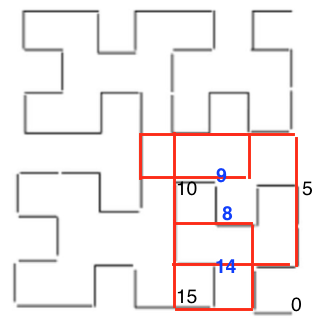
\includegraphics[]{images/hilbert_value.png}
			\caption{The third order Hilbert curve fit to the given bounding boxes.}
			\label{hilbert_curve}
		\end{center}
	\end{figure}		
		
		\item 
		\item
	\end{enumerate}
\section{Trajectory analysis}
	\begin{enumerate}[a)]
		\item The solution for both tasks can be found in the attached $trajectory\_analysis.R$ file. 
		
		\item The $douglasPeucker()$ function simulates the Douglas-Peucker algorithm on the provided trajectory. With the error bound of 0.005 units, the algorithm senses two points as shown on Figure \ref{douglas_peucker}. This yields in a reduction rate of $749 / 2 = 374.5$.
		
		\begin{figure}[h] 
		\begin{center}
			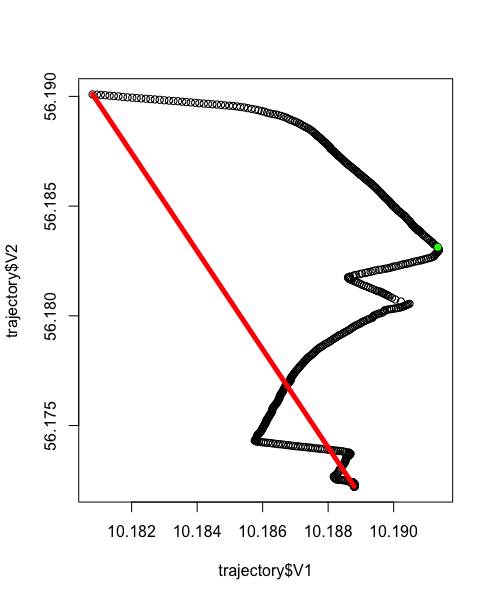
\includegraphics[width=0.5\textwidth]{images/douglas-peucker-1.png}
			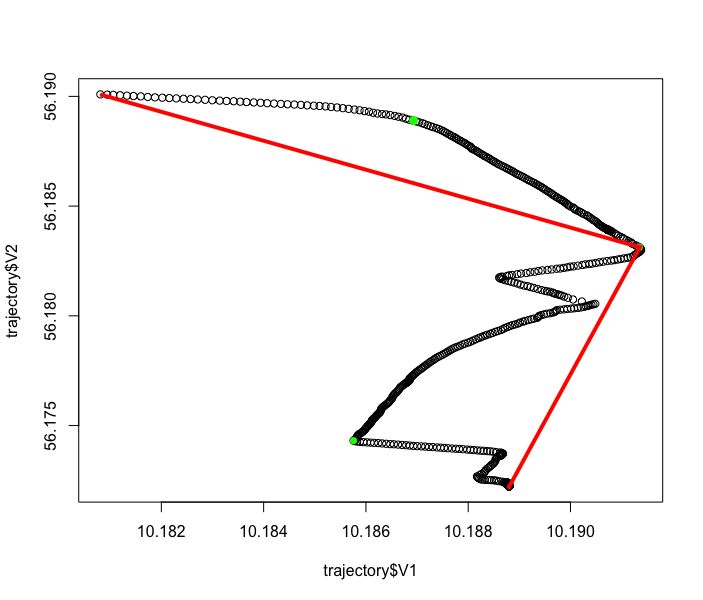
\includegraphics[width=0.5\textwidth]{images/douglas-peucker-2.png}
			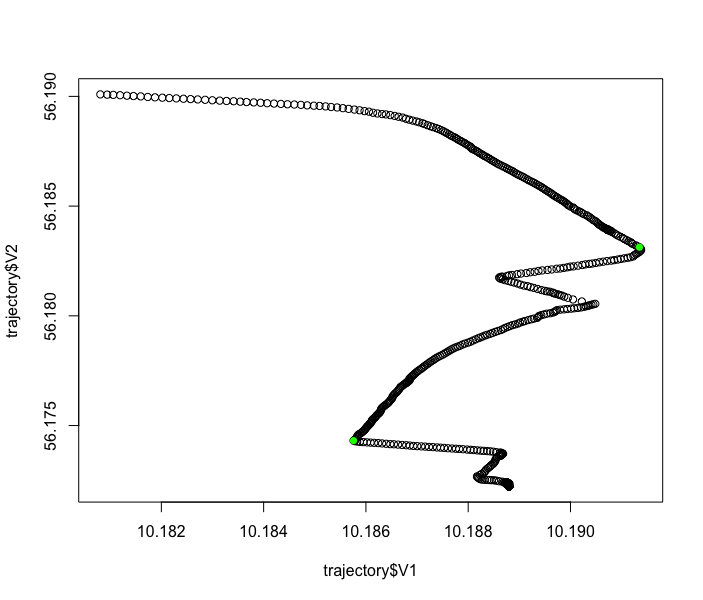
\includegraphics[width=0.5\textwidth]{images/douglas-peucker-3.png}
			\caption{The three steps of the Douglas-Peucker algorithm on the given input. As shown, sensing two points was sufficient enough to match the 500 meter error rate.}
			\label{douglas_peucker}
		\end{center}
	\end{figure}		
	\end{enumerate}

\section{Transportation modes}
	\begin{enumerate}[a)]
		\item The values are calculated by the $transportation\_modes.R$ script. The values for the given dataset using the given thresholds are as follows. As the assignment suggested, 1 km was used as a unit distance for the calculations. 
		
		\begin{eqnarray*}
			d = 327.1344 \\
			\\
		 	|P_c| = 8 \rightarrow HCR= |P_c| / d = 24.45478 \\
		 	|P_s| = 2 \rightarrow SR = |P_s| / d = 6.113695 \\
		 	|P_v| = 39 \rightarrow VCR = |P_v| / d = 119.2171
		\end{eqnarray*}
		
		\item To tell the motion of the measurements, the mean variance and intensity was calculated. The findings suggest that the data in $mode1.csv$ was recorded while the user was standing still and the data in $mode2.csv$ was recorded on the tram while moving. Table \ref{Intensity-and-variance} summarizes the findings.
		
		\begin{table}[]
			\centering
			\caption{The mean intensity and variance of the provided measurements.} 
			\label{Intensity-and-variance}
			\begin{tabular}{llll}
			\\
			\hline
          & Mean intensity & Mean variance & Conclusion     \\ \hline
			mode1.csv & 1884.4         & 11.90095      & Standing still \\
			mode2.csv & 1830.4         & 14.21143      & Moving         \\ \hline
			\end{tabular}
		\end{table}
		
	\end{enumerate}

\section{Temporal modeling}
	\begin{enumerate}[a)]
		\item The solution is implemented in the attached $temporal\_modelling.R$ script file. More specifically, the $discretizeData()$ function performs the calculation of seconds since midnight for each timestamp and performs the bin-categorization accordingly based on 15-minute slots. 
		\item 
		\item
	\end{enumerate}
	
\nocite{*}
\bibliographystyle{tktl}
\bibliography{lahteet}

\lastpage

\pagestyle{empty}

\end{document}